\documentclass{article}\usepackage[]{graphicx}\usepackage[]{color}

\usepackage{alltt}
\usepackage{float}
\usepackage{graphicx}
\usepackage{tabularx}
\usepackage{siunitx}
\usepackage{amssymb} % for math symbols
\usepackage{amsmath} % for aligning equations
\usepackage{textcomp}
\usepackage{booktabs}
\usepackage{mdframed}
\usepackage{natbib}
\usepackage{comment}
\usepackage{booktabs}
\usepackage[colorinlistoftodos]{todonotes} % to make comments on the margin
\usepackage[small]{caption}
\setlength{\captionmargin}{30pt}
\setlength{\abovecaptionskip}{0pt}
\setlength{\belowcaptionskip}{10pt}
\topmargin -1.5cm        
\oddsidemargin -0.04cm   
\evensidemargin -0.04cm
\textwidth 16.59cm
\textheight 21.94cm 
%\pagestyle{empty} %comment if want page numbers
\parskip 7.2pt
\renewcommand{\baselinestretch}{1.5}
\parindent 0pt
%\usepackage{lineno}
%\linenumbers

%% R Script

\title{Unravelling the phenology-phylogeny tangle.}

% alternative titles:
%% An expanded bayesian phylogenetic mixed model to unravel the phenology-phylogeny tangle. %% this sounds too methodsy

\begin{document}

\maketitle

\noindent Authors:\\
The Wolkovich Lab in 2019 \& collaborators $^{1,2,3,4}$ % Will Pearse, Jonathan Davies also
\vspace{2ex}\\
\emph{Author affiliations:}\\
$^{1}$Forest \& Conservation Sciences, Faculty of Forestry, University of British Columbia, 2424 Main Mall, Vancouver, BC V6T 1Z4;\\
$^{2}$Arnold Arboretum of Harvard University, 1300 Centre Street, Boston, Massachusetts, USA;\\
$^{3}$Organismic \& Evolutionary Biology, Harvard University, 26 Oxford Street, Cambridge, Massachusetts, USA;\\
$^{4}$Edificio Ciencias, Campus Universitario 28805 Alcalá de Henares, Madrid, Spain\\
 

\vspace{2ex}
$^*$Corresponding author: ignacio.moralesc@uah.es\\
\renewcommand{\thetable}{\arabic{table}}
\renewcommand{\thefigure}{\arabic{figure}}
\renewcommand{\labelitemi}{$-$}
\setkeys{Gin}{width=0.8\textwidth}

%%%%%%%%%%%%%%%%%%%%%%%%%%%%%%%%%%%%%%%%%%%%%%%
%%%%%%%%%%%%%%%%%%%%%%%%%%%%%%%%%%%%%%%%%%%%%%%
\clearpage



%%%%%%%%%%%%%%%%%%%%%%%%%%%%%%%
% Results & Discussion
%%%%%%%%%%%%%%%%%%%%%%%%%%%%%%%

%%%%%%%%%%%%%%%%%%%%%%%%%%%%%%%
% Discussion
%%%%%%%%%%%%%%%%%%%%%%%%%%%%%%%

%\section*{Discussion}
% EMW (26Apr2022): Some great text here! Would flow really well with a combined R&D.
%IMC 06may - Giving a try at merging Results and Discussion below


\section*{Results \& Discussion}

Most species are sensitive to all three primary cues---forcing, chilling, and photoperiod (Figs. \ref{fig:muplot_all}, Supporting Table \ref{tab:})\citep[see also][]{Laube:2014aettinger2020}(Flynn&Wolkovich)---but with sensitivity to chilling approximately five-fold greater than sensitivity to photoperiod, on average (phenological advances of 7.2 days per standardized unit vs 1.4 days, for chilling and photoperiod, respectively; see Table \ref{tab:modelanglamb}). However, these average sensitivities fail to capture the large differences in species' responses to chilling and forcing (Figs. \ref{fig:muplot_all}, Supporting Table \ref{tab:}). By allowing species responses to vary, we show that the interspecific variation in responses to chilling and forcing is of an even greater magnitude than the average species differences in responses between cues. Robust phenological forecasts must, therefore, account for both the complexity of multiple cues and species-level variation in responses to them.

Clade-wide differenses in the strength of species responses to different cues are striking. For example, oaks and beeches (Fagaceae), elms (Ulmaceae) and buckthorns (Rhamnaceae) are highly sensitive to chilling while rhododendrons (Ericaceae), butterfly bushes (Scrophulariaceae) or spindles (Celastraceae) show little to no response to chilling (Fig. \ref{fig:muplot_all} a). %IMC: not sure if we need some natural history here or some mention to research for some of these clades. Lizzie, if you want to mention-cite something here, please jump in. % EMW (21Nov2022) I'll add more here later.
% JD I think some biogeography may be useful here, for example, I think rhododendrons & buddleia are natve to the Himalaya, but both are also now widespread and invasive ... need to do a little more digging on the extact species.   
Similar clade-level variation is observed for forcing, where some of these clades---e.g., Ericaceae, Rhamnaceae, Ulmaceae, or Fagaceae---are particularly sensitive (advancing their budburst more than 10 days per standardized unit of forcing) and others such as the Sapindaceae, Cornaceae or Juglandaceae families show little response (Fig. \ref{fig:muplot_all} b).\\ %JD - perhaps could link back to invasiveness? Species more sensitive to forcing more invasive?
In contrast to both chilling and forcing, species-level responses to photoperiod are almost uniform, departing from some earlier analyses (e.g. Hunter & Lechowicz (1992); Schaber & Badeck (2003)). Evidence for advances in timing of budburst and flowering with recent warming indicate that photoperiod does not strongly constrain spring phenology (cite: https://onlinelibrary.wiley.com/doi/full/10.1111/pce.12431); nonetheless, our results suggest that while chilling and forcing are the dominant cues by the magnitude of their effect sizes, most species are also sensitive to photoperiod (see also: https://onlinelibrary.wiley.com/doi/full/10.1111/pce.12431). In plants, photoperiod regulates a number of fundamental processes including growth, flowering, stress tolerance, and circadian rhythm (cite: Serrano-Beuno 2017:  https://doi.org/10.1016/j.pbi.2017.03.007), and photoperiodic sensing and adaptation to shifting daylength likley occurred early in the evolution of plants, with origins in the green algae (cite: Serrano-Beuno 2017:  https://doi.org/10.1016/j.pbi.2017.03.007). It is possible, therefore, that phenologial responses to photoperiod reflect ancestral sensitivities with origins in deep time. Large plasticity in responses to additional environmental cues for a given photoperiod cue (e.g. Kramer 1995, Phenotypic plasticity of the phenology of seven European tree species, in relation to climatic warming) may allow species to track interannual variation in climate with little directional selection on photoperiod sensitivities.\\
%JD - I still need to get to grips with what is going on with photoperiod, low lambda is consistent with rapid evolution within species, but low sigma suggests low rates of evolution. Perhaps photopeiod is dominated by local adaptation, but little directional selection, so local adaptation just gets washed out overtime?
%Alternatively, photoperiod might thus provide a reliable calibration of the underlying biological clock \citep{jackson2009plant} upon which seasonal variation in climate modifies the tempo. 

Some species respond strongly to both chilling and forcing, which could suggest the existence of syndromes where the genetic basis for responses to one cue (e.g., forcing) could have been selected for along with responses to another cue (e.g. chilling). We might expect, for example, early season species to be sensitive to multiple cues as mistiming phenology could result in exposure to harsh conditions, leading to tissue loss or death of plants (cite?), and sensitivity to multiple cues likely provides greater insurance against mistiming (cite? Pau et al.?). It is also possible that there may be linkage or pleiotropism among loci associated with sensitivity to different cues (cite: https://link.springer.com/article/10.1007/s00122-004-1905-4). However, the correlation in species senstivities across cues is only weak (\emph{r} = 0.31; between forcing an chilling) and some genera, such as \emph{Tilia} and Ericaceae[genus?], display strong responses to forcing but weak responses to chilling, while others, such as XXXXExamplesXXXX, show strong responses to chilling but weak respones to forcing (Fig. \ref{fig:muplot_all}). Species sensitivity to one cue, thus, do not constrain their senstivities to another cue, and selection might operate independently on responses to different cues (cite?).\\

Our modelling approach not only allows us to quantify individual species responses, it also provides information on the evolution of those responses across the phylogeny. Consistent with previous work showing phylogenetic signal in plant phenology (Davies et al.; Rafferty; etc.), we find responses to all three cues are phylogenetically structured, but the strength of phylogenetic conservatism in responses differs between cues (Fig. \ref{fig:phylosig_all}). Responses to forcing and chilling are strongly to moderately structured($\lambda = 0.65$ and $\lambda = 0.54$, for forcng and chilling, respectively), with closely related species exhibiting more similar sensitivites than distantly related species. We observe weaker phylogenetic structure in species responses to photoperiod ($\lambda= 0.39$) (see Fig. \ref{Fig:muplot_all}, Table \ref{tab:modelanglamb}), emphasising once more that photoperiod (or how we meaure it) diverges from other climate cues. Sensitivity to photoperiod is weaker, more uniform across species, and appears to be less evolutionarily constrained than sensitivities to temperature cues. Helpfully, the contrasts between temperature sensitivities and phptoperiod sensitivities in both their variability across species and phylogenetic structuring allow for improved multi-species forecasts: (1) the large variability among species in tempertaures responses makes predicting species individual responses challenging, but the phylogenetic structure in responeses lets us borrow  information from close relatives to imporve our predictions; (2) the weak phylogenetic stucture in photoperiod responses indicates that phylogeny retains little information, but because species responeses are generally more uniform, we can be more confident in assuming the mean species repsonse across species, comforted in the knowledge that small errors will likley not have large impact given the realtively weak overall contribution of this cue. 
\\

What might drive phylogenetic structure in species temperature responses? Within our statistical modelling framework, differences in species responses represent shifts in the slope of the relationship between the observed pehnology and the cue. Phylogenetic structure in the change in slope across the phylogeny would be consistent with an interaction with a non-measured trait that moderates species sentivities, and which also covaries with phylogeny (cite PWR). Our results indicate the presence of important modifiers for responses to chilling and forcing. Plant life history traits (citeXXX) provide a source of likely modifiers; early season species with fast life histories ... late season species .... Geography may be an additional source of structured variation, especially in regions where clades have radiated such that close relatives will have been expposed to the same suite of environmental cues and thus subject to similar selection regimes. Conversely, if species are not generally geographically constrained, as may be more likley the case, especially across deep time ( https://doi.org/10.1111/j.0014-3820.2006.tb01140.x), then we might expect phylognetic structure in phenology to also weaken, especially when aggregating across locations with different cues (citeXXX Davies phylo sig paper?).
\\

% EMW (21Nov2022): Do we want to mention any molecular work on photoperiod (or other cues)?
Weak phylogenetic signal in photoperiod sensitivity (Fig. \ref{fig:phylosig_all}) might seem at odds with observations that distantly related species respond more similarly (and less variably) to photoperiod than they do to forcing or chilling. However, somewhat counterintuitively, both uniform and random responses can manifest as low phylogenetic signal when indexed by Brownian motion expectations (see Wiens et al.). Rapid local adapatation within species might thus erase the phylogenetic stucture in photoperiod responses, but would seem at odds with the uniformity in species' responeses. Alternatively, if responses to photoperiod evolved early in plants, as we suggest above, and subsequent selection on photoperiod sensitivity was constrained by stabilising selection operating on other life-history attributes senstive to photoperiod (XXCITE), we would predict both low interspecific variation and weak phylogenetic signal in responses, matching observations. This latter interpretation is also consistent with our estimates of lower $\sigma$ for photoperiod responses (CITE FIGURE). Here, as in more traditional phylogenetic comparative methods, $\sigma$ represents the rate of evolution, and thus our model suggests photoperiod responess are also evolving slower then temperature responses. However, we also reveal (see Appendix XXX) that an early burst model of evolution, in which trait variation accumulates rapidly early in the history of a cladde and then slows through time, consistent with our interpretation of photoperiod evolution.
%JD - Call out to Will for assistance ...
\\

The genus \emph{Fagus} is recognsied as being particularly sensitive to photoperiod \citep{fu2019}. Specifically, \emph{Fagus sylvatica} is nearly five times more sensitive to photoperiod than most other measured tree species. The question arises as to whether species with outlying responses should be chosen as the model from which to extrapolate knowledge as done with \emph{Fagus sylvatica} in the phenology literature (REFs for PEP75?!). \\%HELP with references on Fagus would be appreciated. % EMW (21Nov2022) I'll add more here later
%JD - this para needs a home ... perhaps when we talk about future ofr forecasting ...

Phylogenetic conservatism (high $\lambda$) and slow evolutonary rates (low $\sigma$) in traits has sometimes been interpreted as indicative of evolutionary constraints to adaptive change (cites Wiens et al. and others cites XXX). If this were the case, we might then suggest that species with strong forcing response might be more vulnerable to future warming spring temperatures because phylogenetc signla in resonese to forcing is strong, while species may be able to better adpat to changes in chilling as $\lambda$ is lower, and $\sigma$ is higher. However, this is misleading as estimates of lambda are independent from the rate of evolution, and macoevolutionary rates estimated on phylogeneic trees are integrate across millons of years of evolutonary history, and thus do not necessariy inform us of maxmum posible rates of evolution over shorter timesacles. Indeed, there is accumulating evidence for rapid evolution to warming climate ... (cites XXXX). We highlight these parameter here to improve our understanding of the evolutionary history of species phenological cues, and to underscore the importance of correctly modelling species differences in ecological forecasts. 
\\

% I'm commenting out this bit but leave it here in case we want to mention some of it in methods or an appendinx
%From a statistical perspective, accounting for the effects of phylogenetic structuring on the effects of jointly modelled cues had an effect on model coefficients (Fig. \ref{fig:correls_angio}). Not accounting for phylogeny (or assuming $\lambda$ = 0) biased model coefficients, particularly so for forcing and somewhat less for chilling (Fig. \ref{fig:correls_angio}). Specifically, species sensitivities to forcing and chilling were underestimated on average (model slopes shifted by 7.2\% and 3.7\%, respectively). Sensitivities to photoperiod, which showed weak phylogenetic signal were not biased in non-phylogenetic models (Fig. \ref{fig:correls_angio}), likely associated to their low estimated $\lambda$ values. Model intercepts were not affected either (Fig. \ref{fig:correls_angio}).\\ 


% EMW (21Nov2022): I suggest we drop lamba=1 to keep this short and restructure a little ... maybe something like 'even though average slopes did not change so much ... we saw important changes across species when including the phylogeny' or such? I am happy to work on this after we discuss. 
Not accounting for phylogeny had an effect on model coefficients (model slopes for forcing and chilling shifted by 7.2\% and 3.7\%, respectively; Fig. \ref{fig:correls_angio}) and shifted cross-species variance in their responses to forcing (Var $\beta_{phylo}$ = 8.74; Var $\beta_{non-phylo}$ = 5.01), chilling (Var $\beta_{phylo}$ = 23.45; Var $\beta_{non-phylo}$ = 17.47), and photoperiod responses (Var $\beta_{phylo}$ = 0.82; Var $\beta_{non-phylo}$ = 0.93). Counterintuitively, induced reductions in cross-species variance, far from increasing estimation accuracy could lead to increased type-II error by failing to detect actual relationships among cue and responses that would only emerge when phylogeny is correctly accounted for (see Supporting Information XX). Either ignoring ($\lambda$ = 0) or overestimating phylogenetic structuring of predictors ($\lambda$ = 1) can bias model coefficients (predictors with high $\lambda$ are biased in non-phylogenetic models and those with low $\lambda$ are biased if Brownian Motion is imposed). Importantly, not accounting for phylogeny increased the uncertainty around each individual species estimation of their responses to forcing and chilling (see Fig. SXX in Supporting Information), which could lead to less precise predictions and forecasts of phenology for individual species although overall model accuracy might still appear reasonable (see Appendix XX in Supporting Information).\\
%IMC: I merged and tried to condense these statistical findings. Probably the paragraph can still use some work.

%IMC- I'm commenting out this paragraph as I'm not sure we want to discuss intercepts. in 20nov meeting we decided not to talk about this unless Will feels we should and has something to add to this paragraph.
%Our models found non-negligible phylogenetic signal in model intercepts (see \ref{fig:phylosig_all}). This indicates that the intrinsic variation across species in the timing of budbreak before experiencing the effects of any environmental cue, is also phylogenetically patterned. This is, regardless the action of cues some tree species budbreak earlier than others, and these differences tend to be smaller, at least to some extent (the signal is weak $\lambda$ = 0.35), among closely related species. Previous work had already shown large variation across species in their model intercepts \citep{davies2013phylogenetic}. % not sure this is the right citation, ask Lizzie. This whole paragraph needs work (based on conversation over coffee May6th).  While fitted species-level intercepts did not change between the phylogenetic and non-phylogenetic model (\ref{fig:correls_angio}), our approach suggests that the mechanisms underlying species' baseline phenological differences would not operate randomly across the phylogeny.\\    

Phylogenetic hierarchical models such as those used here, have the potential to inform on which clades will be more sensitive to different axes of climate change---e.g., changes in cold temperatures over winter or in warm temperatures in spring and summer. For example, in standard non-phylogenetic models, we would not have identified oaks (genus \emph{Quercus}) as being among the most sensitive taxa to forcing and chilling (see e.g., \citep{ettinger2020}), but we show that species within this genus advance phenology by 2 days per standard unit of forcing and 4 days per standard unit of chilling. Ignoring phylogeny and species-level variation may (i) introduce bias into estimated model coefficients, (ii) underestimate true variability in species biological responses and, (iii) increase uncertainty around species-level estimates. Our integratve phylogenetic approach allows us to move beyond crude classifications based upon functional groups (e.g., !REFS) and species complexes (e.g. \cite{ettinger2020}), to make improved ecological forecasts for individual species. Our model, highlighting strong phylogenetic structure in species repsonese, also highlights the potential for predicting phenological sensitivities in unmeasured species. While phylogenetic imputation must be done with extreme care \citep{molina2018assessing}, we can make predicions with reasonable accuracy for close relatives of well studied species when there is strong phylogenetic structure in species responss. Notably this is likely to be the case for many temperate woody plant clades, for which we have multiple experimental observations at varying treatment levels for well-known drivers of phenology.\\ 

Accurate forecasts of phenology remain elusive; recent records have suggested an apparent decline in species phenological sensitivity to increasing temperatures \citep{fu2015,piao2017}, but such observations may simply reflect non-linear responses to warming trends \citep{wolkovich2021simple}, perhaps reflecting the complex interactions, trade-offs and synergies among multiple cues. While all species appear sensitive to all cues, forcing and chilling dominating over photoperiod, and species-level variation in responses is large, of a magnitude similar to, or greater than, the difference in average effect sizes between cues. Phylogenetic conservatism in species phenology has been well documented \citep{davies2013phylogenetic,rafferty2017global,joly2019importance}, and may thus help explain species differences. Here, using a novel hierarchical Bayesian model, we allow for phylogenetic non-stationarity in species sensitivities (allowing slopes to vary across species; see \citep{davies2019phylogenetically}) to generate speies-specific estimates of responses to shiftong cues. Uniquely, our model additionally povides information on the evolutionary of species sensitivities, and how they may have been configured along evolutionary time. Our results are consistent with an early origin of photoperiod sensitivity, followed by a history of stabilising selection. Forcing and chilling have evolved more rapidly. However, we caution that macroevolutionary rates provide a poor guide to future adaptive potential over short timescales, and accurate ecological forecasting requires well-designed experiments analysed appropriately.\\


%\subsection*{Model accuracy}
%IMCapr25 - I'd like to include a little subsection here on model accuracy, comparing R2s, LOO, or something similar for our models. Unfortunately, I can't find an easy way to do that (for stanfit objects: https://discourse.mc-stan.org/t/best-way-to-do-prediction-on-new-data-r-rstan-stanfit/1772/17) any help with this is much appreciated. 
% EMW (26Apr2022): To use loo we just need a generated quantities block, right? If so I can try to help code that with Deirdre.
%IMCmay10- I re-run models storing yhats as a generated quantity, and with that computed a Bayes version of R2. There's not change in accuracy between our approach and the lambda0 approach, but accuracy drops if lambda is forced to be equal1. 

%angio
%R2lamb0 0.666
%R2lambest 0.665
%R2lamb1 0.657

%gymno
%R2lamb0 0.527
%R2lambest 0.530
%R2lamb1 0.498



%\item How can we interpret lambdas and sigmas for each cue, and for the intercept?
%\item What are the implications for phenological predictions and forecasts?
%\item Is this approach transferable to different taxa or biological responses? 
%\item Do results differ from what would be expected if single cues where analyzed separately, phylo or non-phylogenetically?


%\item If so, can accounting for phylogeny shed light on the ongoing debate on declining sensitivities? For example, if particular lineages have very different evolutionary constraints on their responses to the cues, they may also display very differt declines in their sensitivities to the cues. % lizzie, I realize I missed important bits on the discussion we had on the relevance of this point, any pointers here are super welcome. 




%\begin{enumerate}
%\item Random discussion points with no home, yet ... 
%\begin{enumerate}
%\item This is a case where phylogeny makes a big difference! Changes overall forcing cues? 
% IMC May6 - sort of dealt with 
%\item Reduced uncertainty in species estimates (I think?) with including phylogeny (goes with above point perhaps also) / % IMC May18 - sort of dealt with 
%\item Even with phylogeny added FagSyl is still freakish for photoperiod cue ... suggesting we've been studying an extreme species as one of our focal species (maybe?) % IMC May18 - this has been dealt with shortly in line 384 (one sentence or so) 
%\item Implications for the declining sensitivities debate? % IMC May18 - done but needs some more work
%\item Highlight/discuss the advantages of pushing methodologies such as the one here % IMC May18 - done but needs some more work




\begin{comment} % I'm pasting this bit from previous version of the intro in case we want to reuse some.
% \item most efforts are on the phenotype rather than on the magnitude of species phenological responsiveness to different environmental cues. 
% Could try to integrate this point above into above paragraph or include in below section that I have commented out ... I think the intro is likely long enough without the below and many of the points could fit in discussion, but up to you!
\iffalse
\item Focused on flowering (and leafout some) times and shifts in them (but see \cite{joly2019importance}, and add REFs!! on other phenological stages: budburst, ripening)
\item Studied trait correlation \citep{bolmgren2008time} (not a limitation, but a different focus)
\item Studied different evolutionary models best fitting the data \citep{rafferty2017global}
\item measured shifts based on field observation data for both climate and phenology (when slopes are available, they represent shifts with time, not shifts with the environment).
\fi
\end{comment}


\bibliography{phylorefs}
\bibliographystyle{amnat}

%%%%%%%%%%%%%%%%%%%%%%%%%%%%%%%
% Tables and Figures
%%%%%%%%%%%%%%%%%%%%%%%%%%%%%%%
\section*{Tables and Figures} 


%IMC 22mar - we should decide among one of the next two figures, instead of having separate figures per cues?
% EMW (28Mar2022): I vote for the first one, but both are great!
\begin{figure} [H]
  \begin{center}
  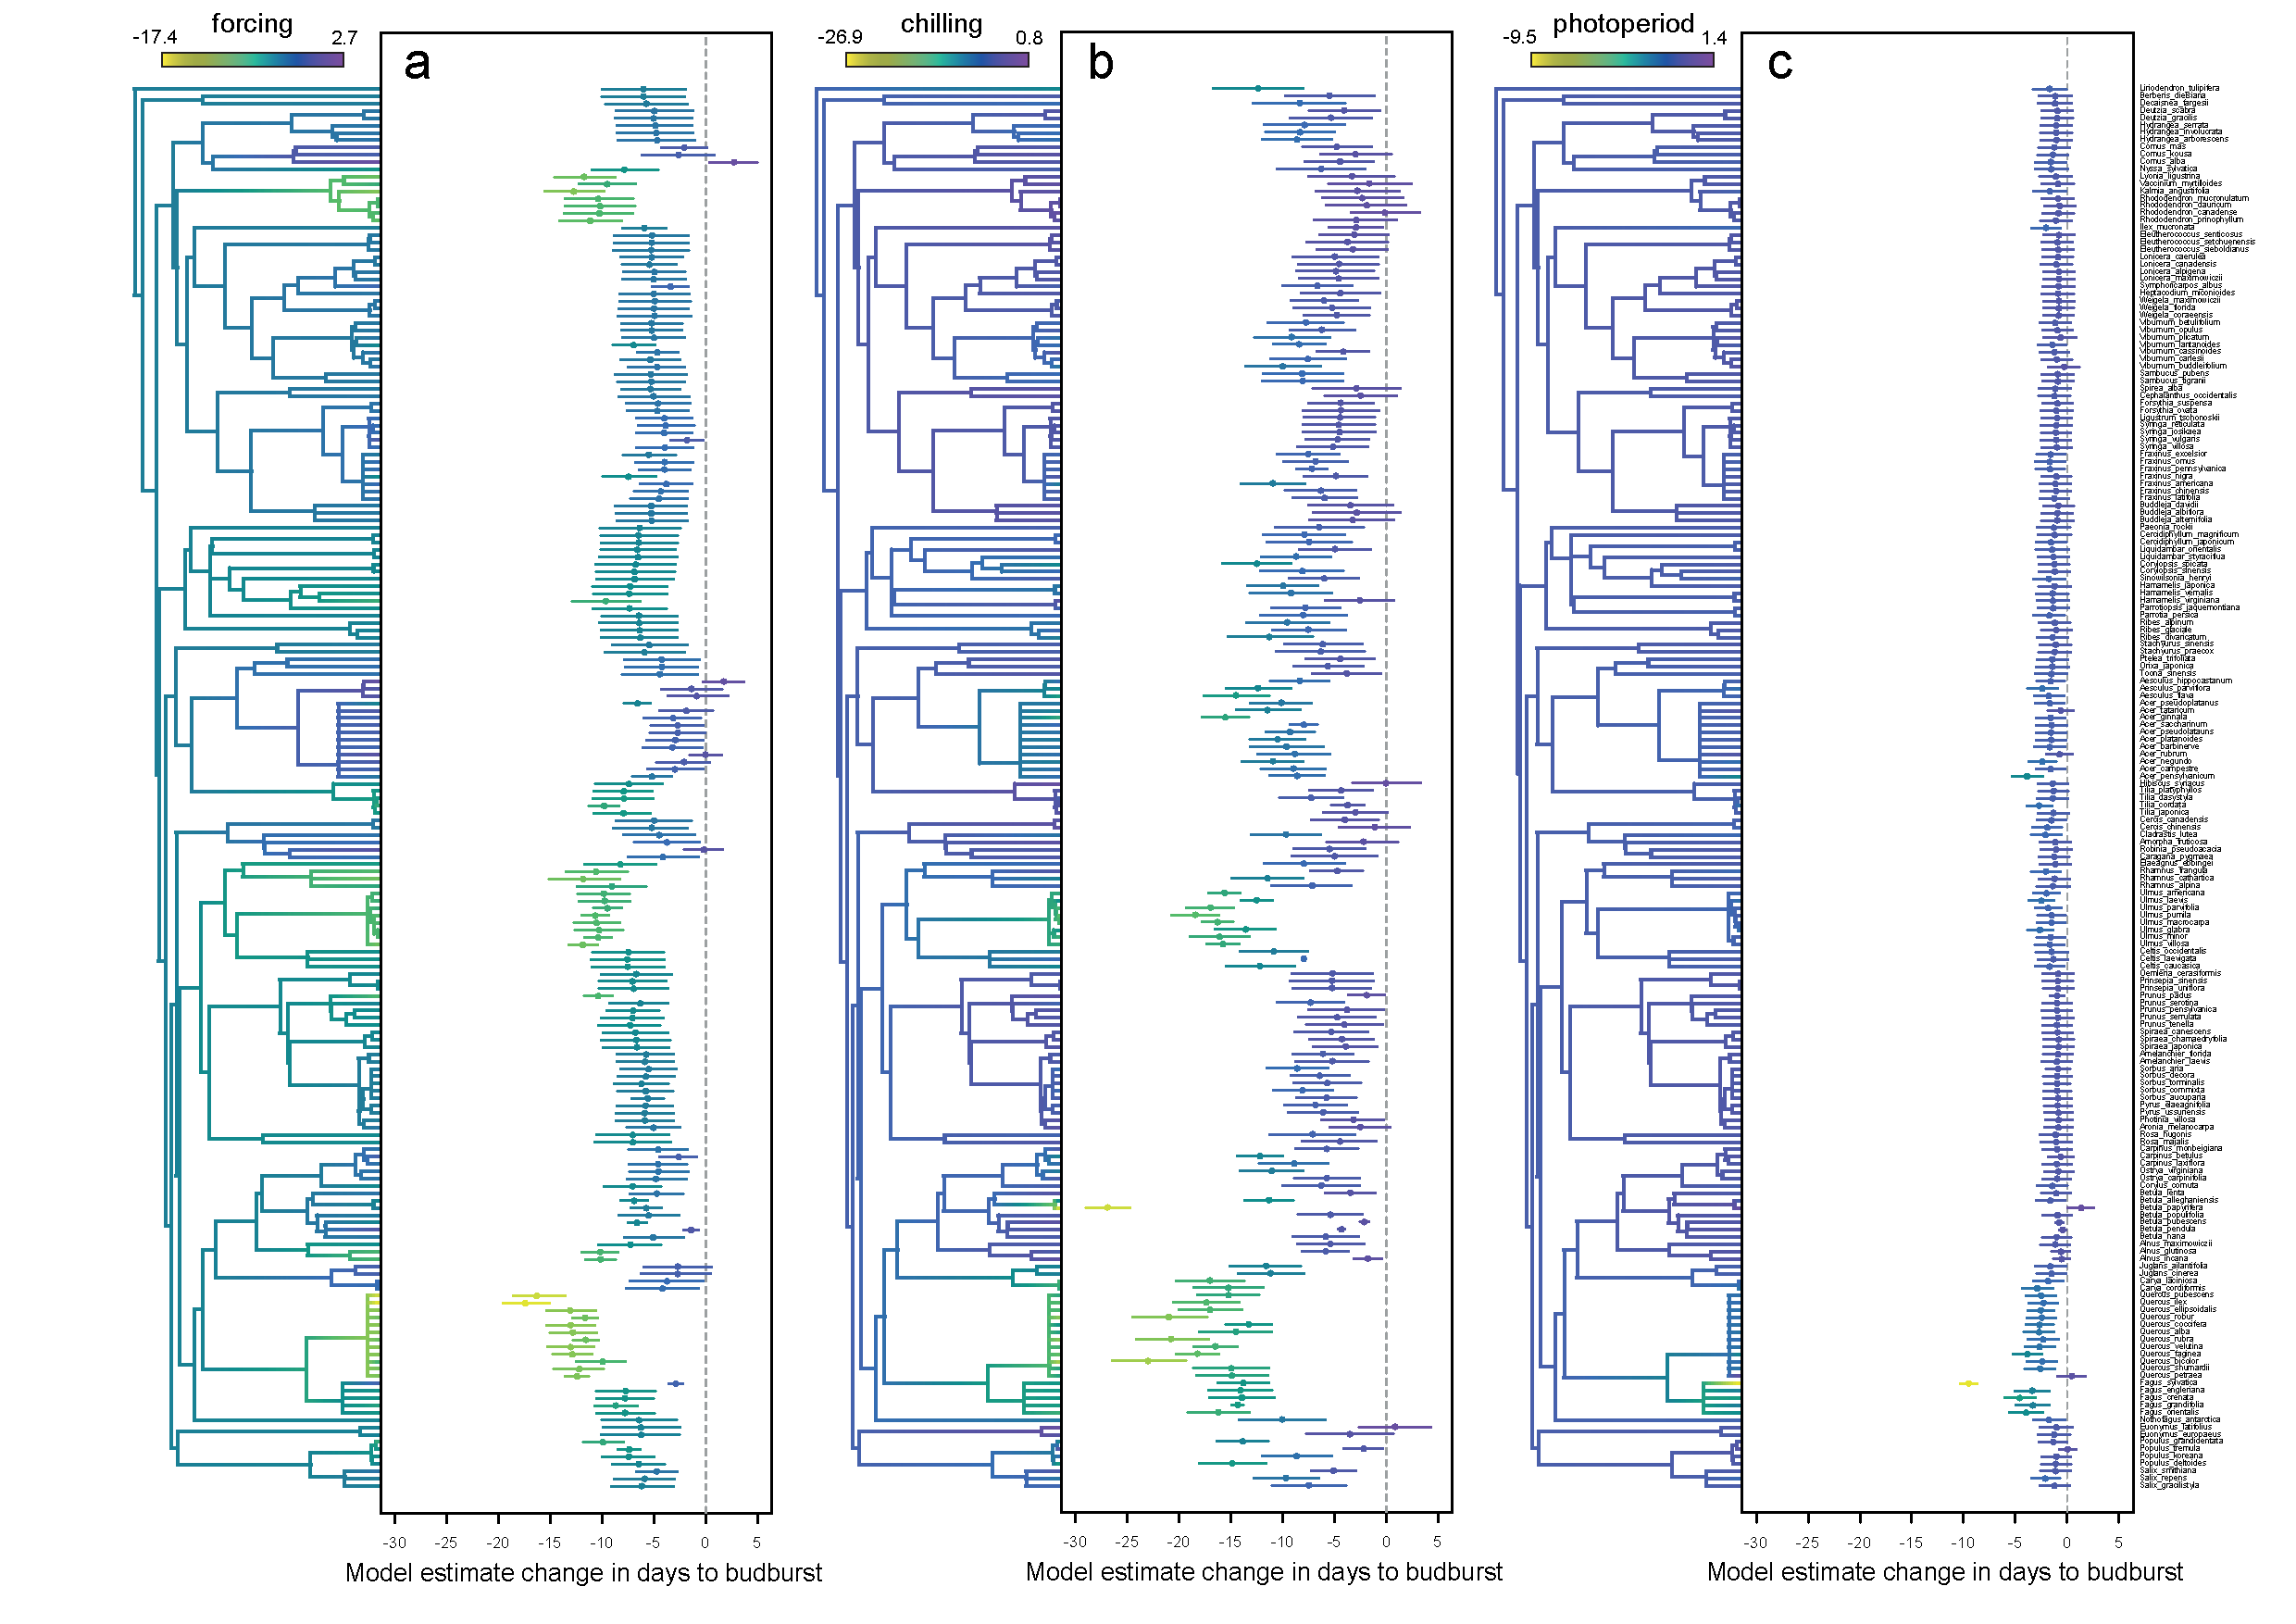
\includegraphics[width=16cm]{../../analyses/phylogeny/figures/muplot_phylo_allcue_angio.pdf}
  \caption{Phenological sensitivity to thee environmental cues, forcing (a), chilling (b) and photoperiod (c) measured in change in days to budburst per standardized unit (z-transformation) of the cues across 192 angiosperm species. The same phylogenetic tree is shown in each panel, colored acording to an estimation of ancestral character states, being the states at the tips the model slopes of our hierarchical phylogenetic model. Note that the color scale varies in each panel. Total tree depth is 81. My.}
  \label{fig:muplot_all}
  \end{center}
\end{figure}

\begin{figure} [H]
  \begin{center}
  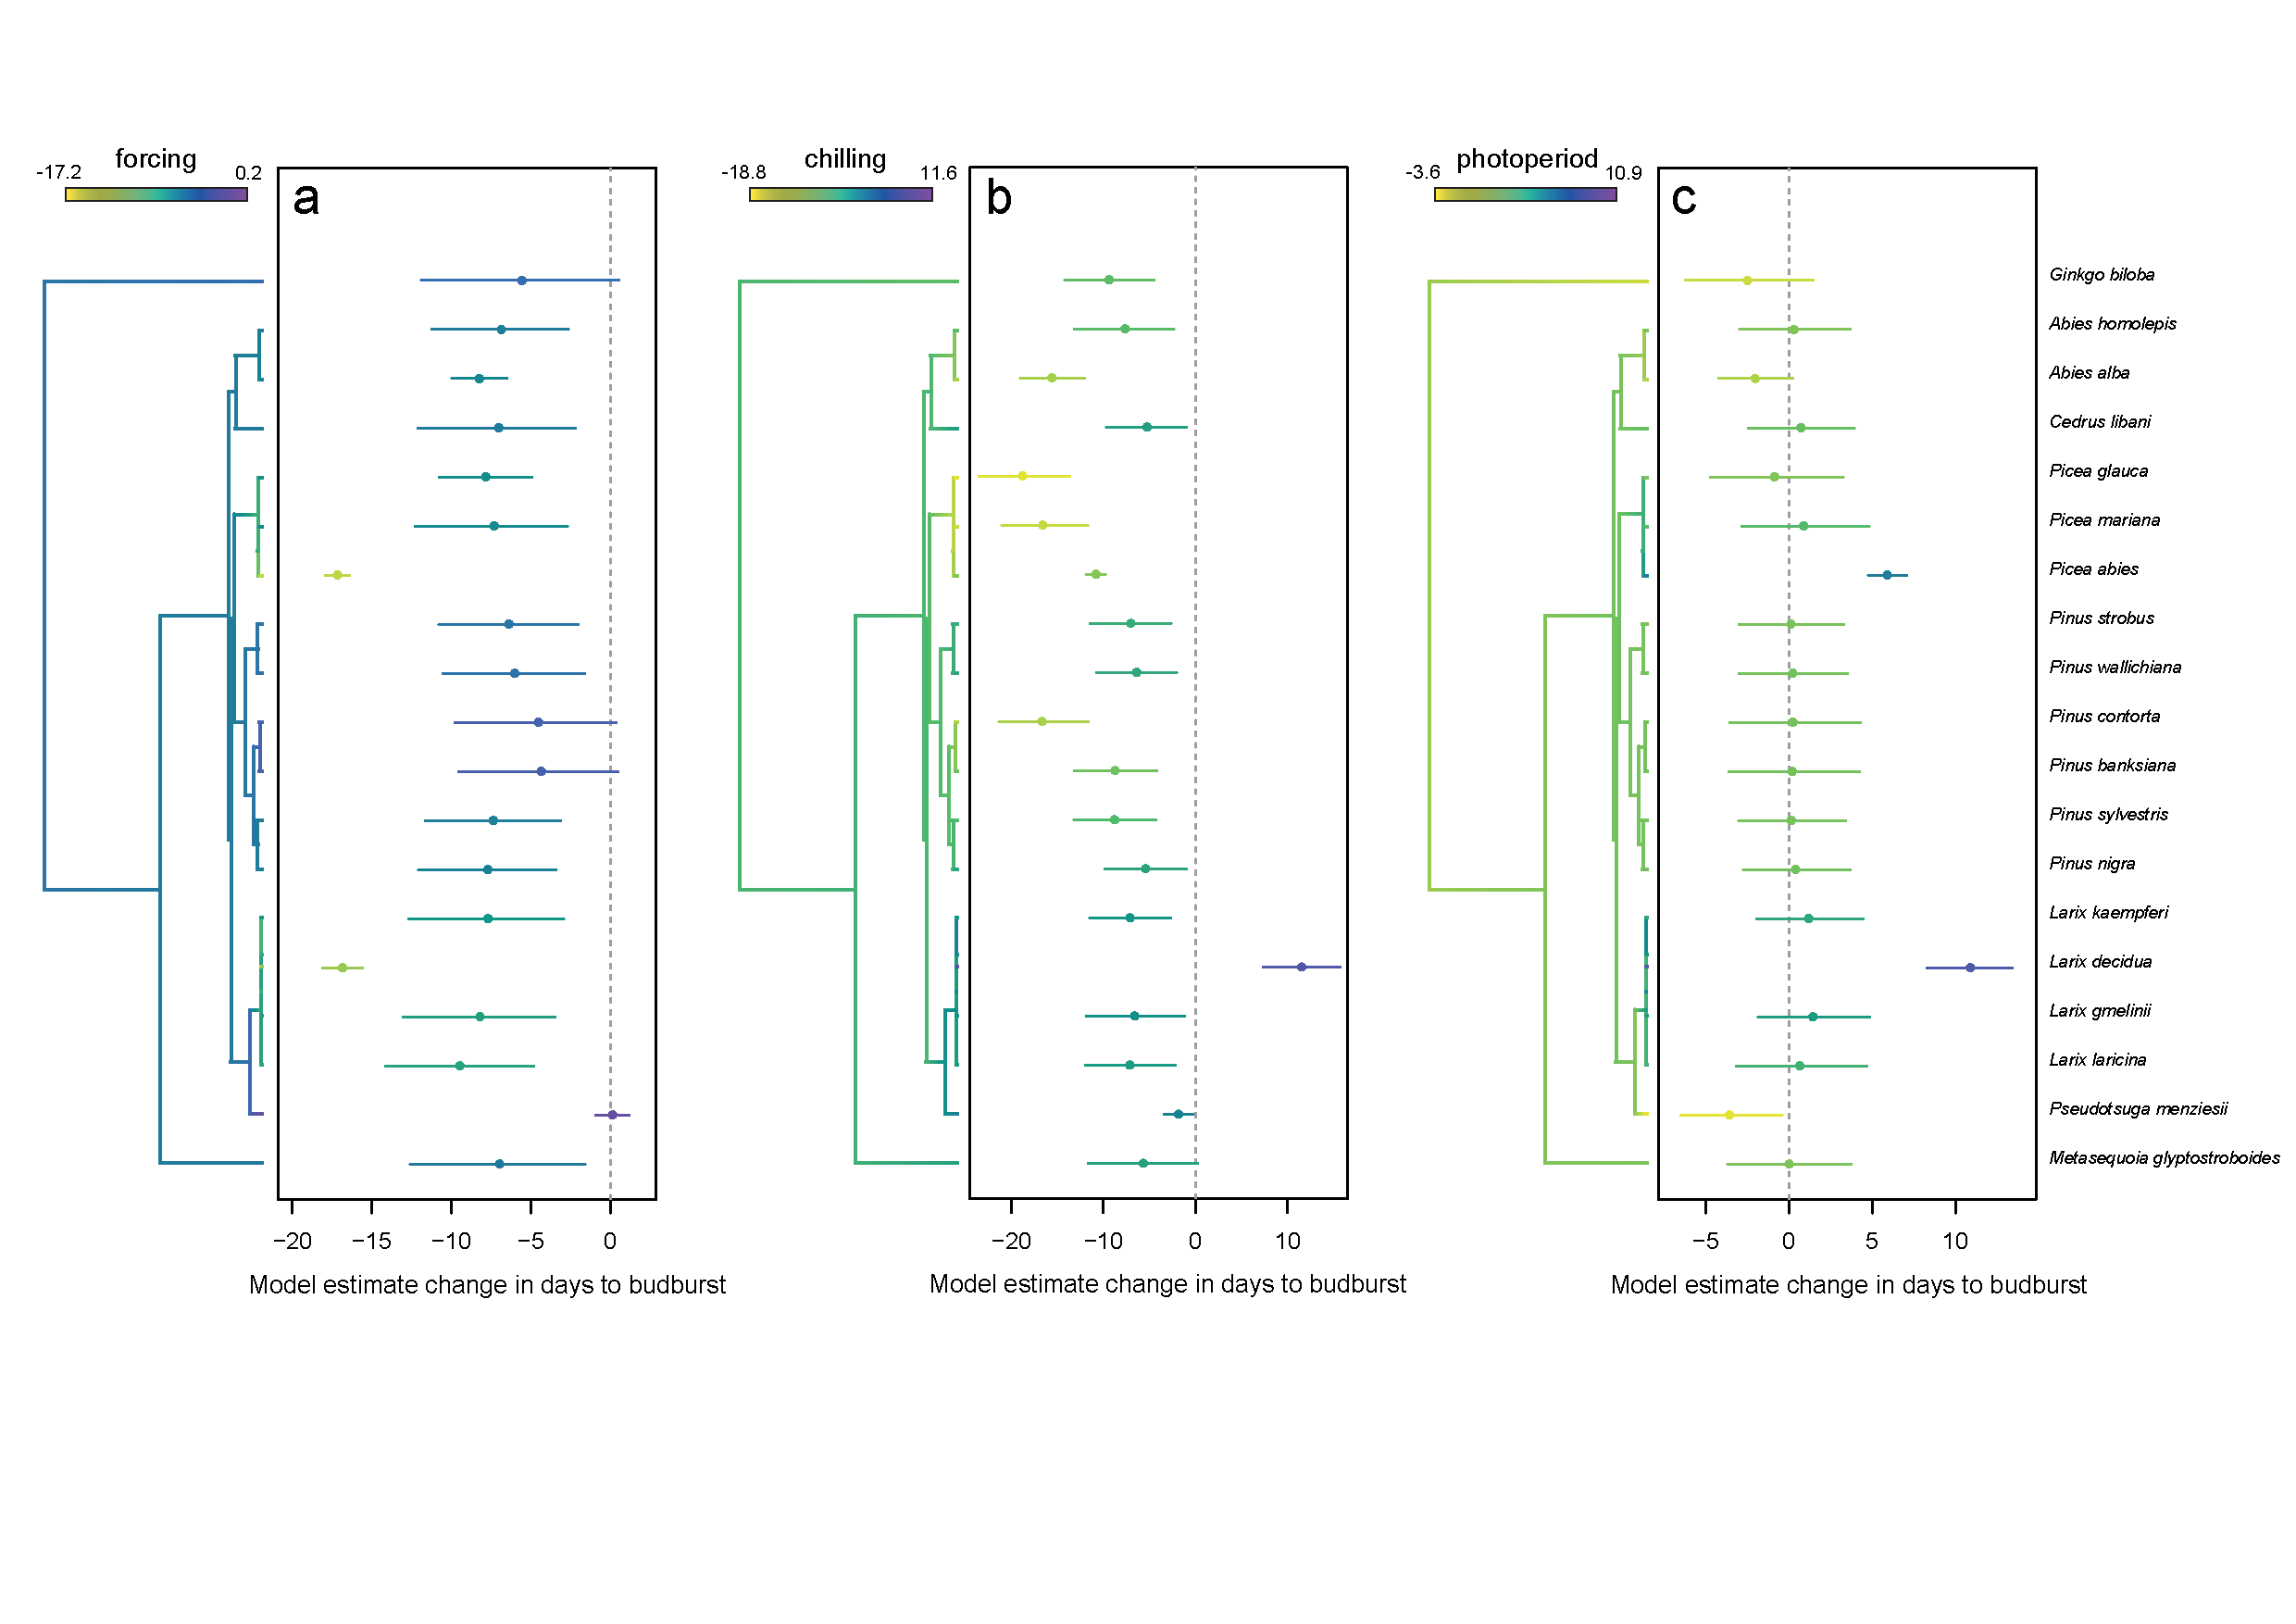
\includegraphics[width=16cm]{../../analyses/phylogeny/figures/Fig1b_phylo_muplots_gymno.pdf}
  \caption{Phenological sensitivity to thee environmental cues, forcing (a), chilling (b) and photoperiod (c) measured in change in days to budburst per standardized unit (z-transformation) of the cues across 19 gymnosperm species. The same phylogenetic tree is shown in each panel, colored acording to an estimation of ancestral character states, being the states at the tips the model slopes of our hierarchical phylogenetic model. Note that the color scale varies in each panel. Total tree depth is 81. My.}
  \label{fig:muplot_allgymno}
  \end{center}
\end{figure}


\begin{figure} [H]
  \begin{center}
  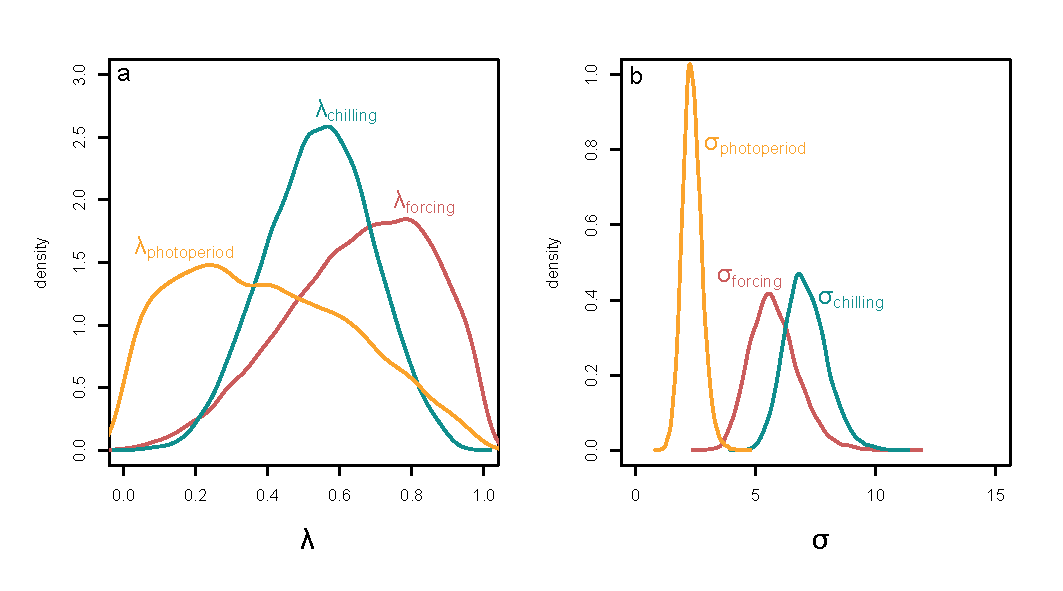
\includegraphics[width=14cm]{../../analyses/phylogeny/figures/Fig2_lambdas_sigmas.pdf}
  \caption{Density plots for the posterior distribution of phylogenetic signal measured by lambda for each cue included as a predictor in the model for angiosperms: forcing (red), chilling (blue),  photoperiod (orange) and for the model intercept (grey). Panels correspond to angiosperms (a-d) and gymnosperms (e-h). Note that lambda estimations corresponding to  panels c-d and g-h as they are constrained to be either equal zero or equal 1.}
  \label{fig:phylosig_all}
  \end{center}
\end{figure}

\begin{figure} [H]
  \begin{center}
  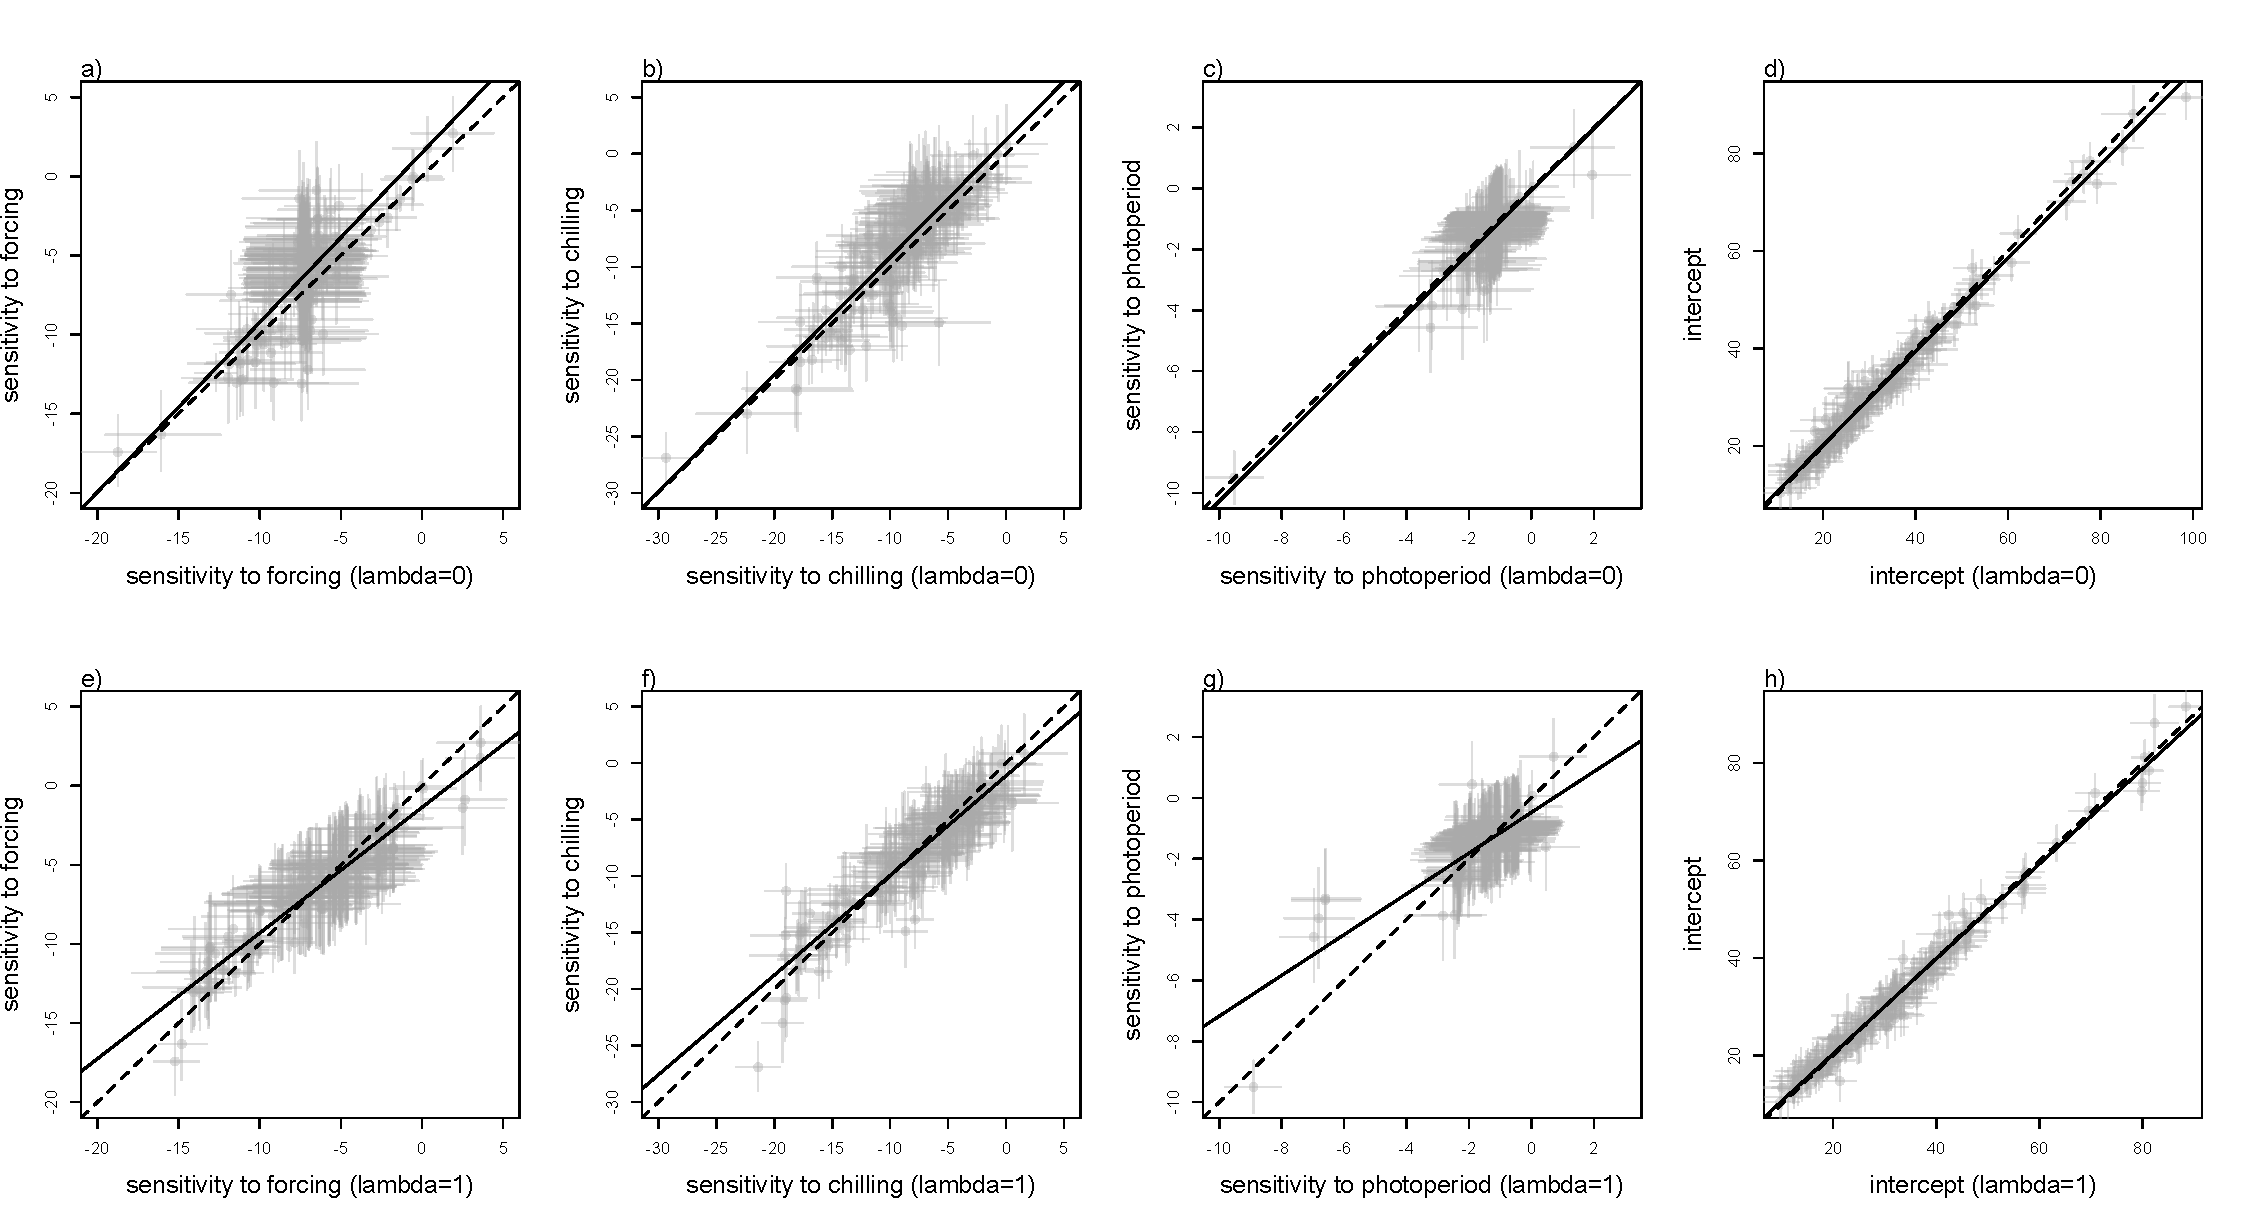
\includegraphics[width=14cm]{../../analyses/phylogeny/figures/Est_correls_vs_lamb01_angio.pdf}
  \caption{Correlations between model parameters as estimated by the full model and the models where lambda is constrained to be equal zero (upper row) or one (bottom row), for angiosperms. Panels correspond to sensitivity to forcing (a,e), to chilling (b,f), to photoperiod (c,g) and to model intercepts (d,h).}
  \label{fig:correls_angio}
  \end{center}
\end{figure}

\begin{figure} [H]
  \begin{center}
  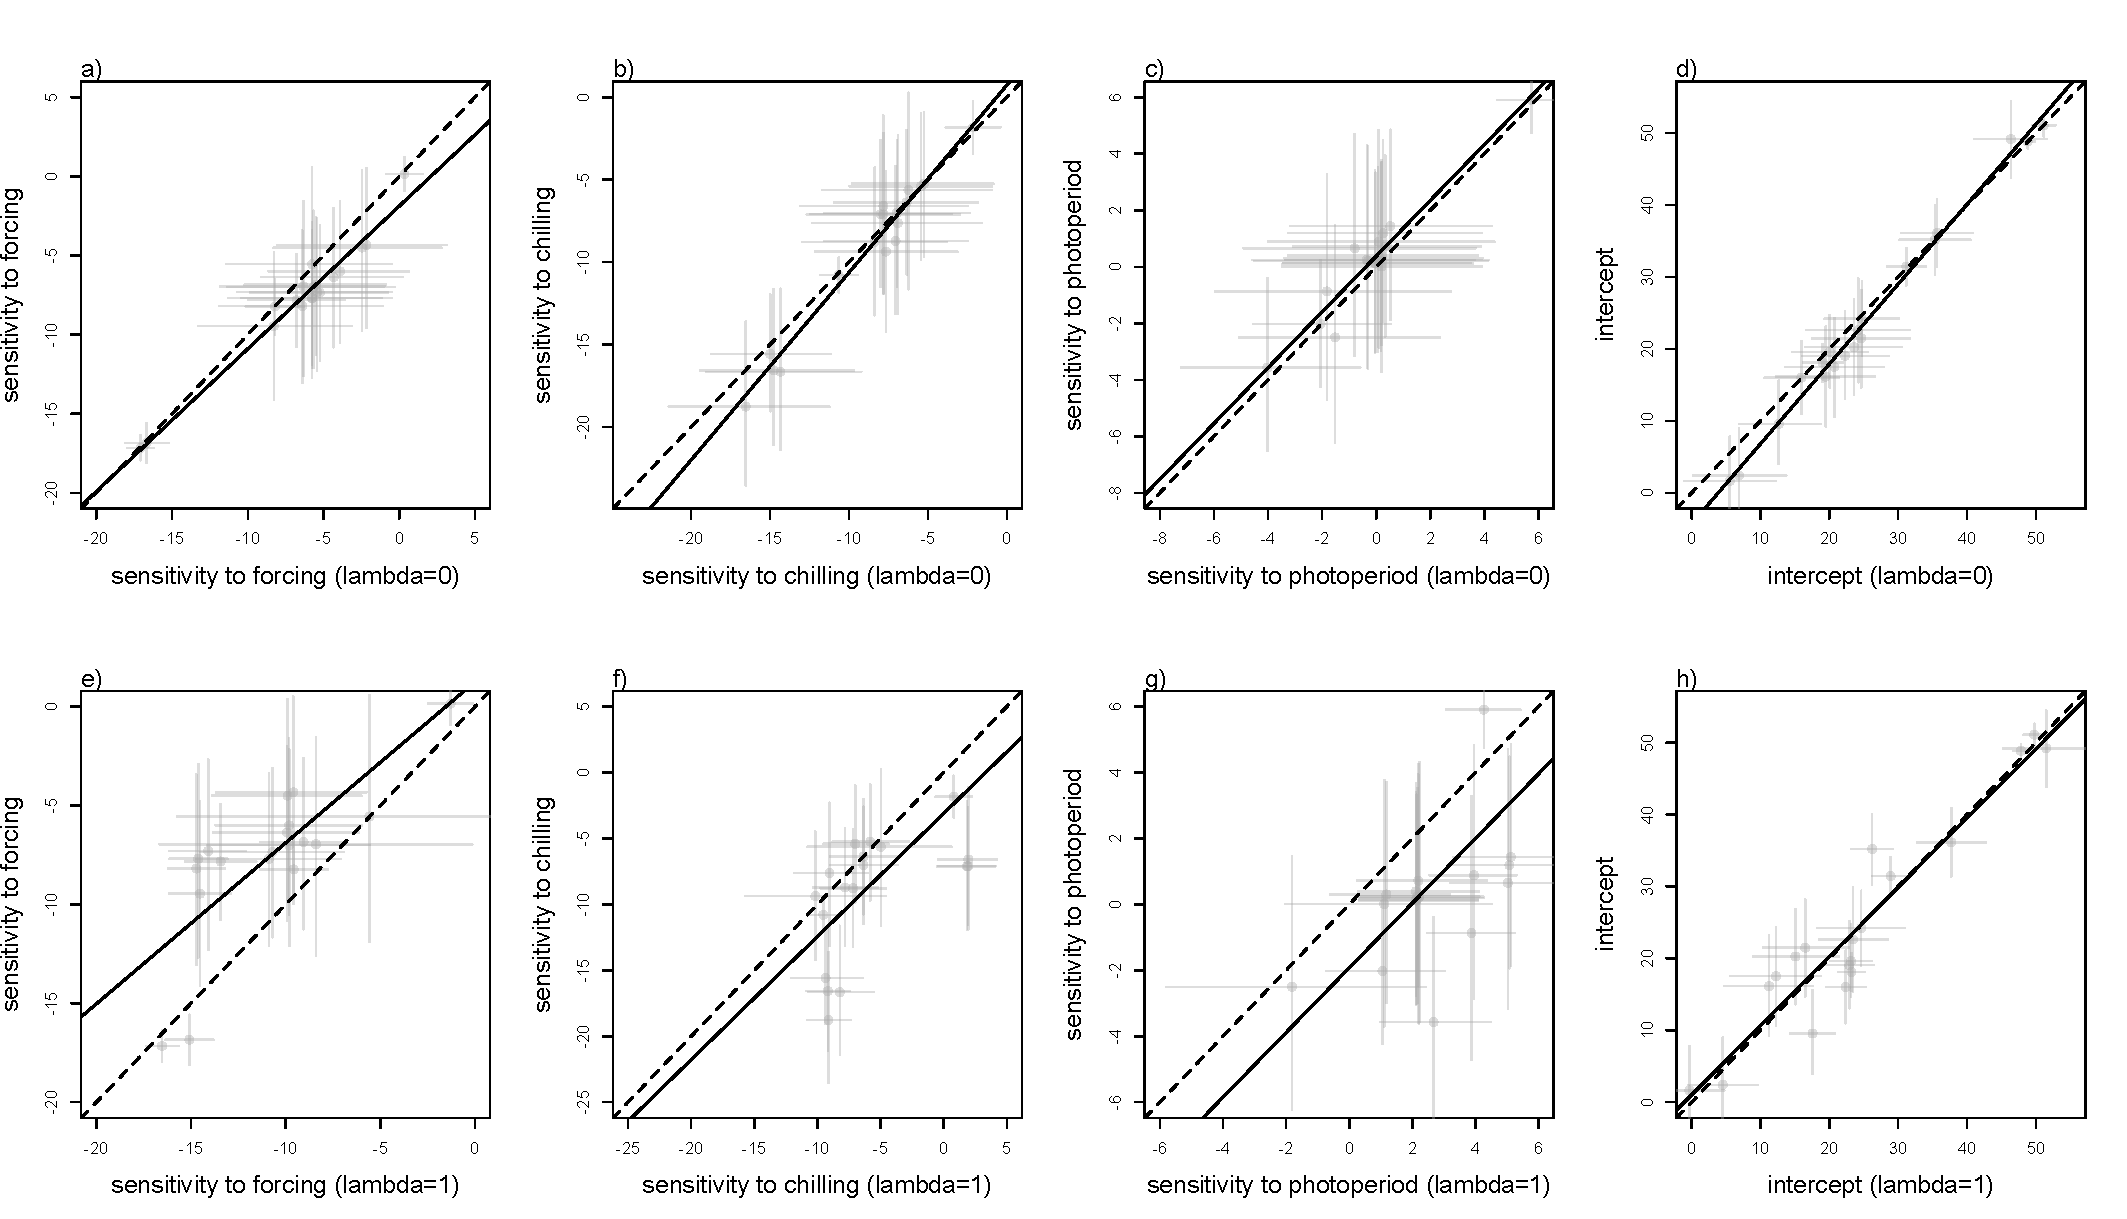
\includegraphics[width=14cm]{../../analyses/phylogeny/figures/Est_correls_vs_lamb01_gymno.pdf}
  \caption{Correlations between model parameters as estimated by the full model and the models where lambda is constrained to be equal zero (upper row) or one (bottom row), for gymnosperms. Panels correspond to sensitivity to forcing (a,e), to chilling (b,f), to photoperiod (c,g) and to model intercepts (d,h).}
  \label{fig:correls_gymno}
  \end{center}
\end{figure}



% IMC Mar21 - I'm guessing we are going to merge some of the tables below. TBD what we keep for the main text and what is sent to a supp.
\begin{table}[H]
\begin{center}
\caption{Full model parameters estimated for 192 angiosperm species.}
\begin{tabular}{@{}lcccccc@{}}
\toprule
\textbf{parameter}             & \multicolumn{1}{l}{\textbf{mean}} & \multicolumn{1}{l}{\textbf{sd}} & \multicolumn{1}{l}{\textbf{2.50\%}} & \multicolumn{1}{l}{\textbf{50\%}} & \multicolumn{1}{l}{\textbf{97.50\%}} & \multicolumn{1}{l}{\textbf{n\_eff}} \\ \midrule
$\mu_\alpha$                   & 30.57                             & 3.41                            & 23.68                               & 30.59                             & 37.14                                & 5031.19                             \\
$\mu_\beta_{forcing}$          & -5.84                             & 2.01                            & -9.72                               & -5.89                             & -1.79                                & 2374.73                             \\
$\mu_\beta_{chilling}$         & -7.19                             & 2.03                            & -11.15                              & -7.18                             & -3.18                                & 3694.93                             \\
$\mu_\beta_{photoperiod}$      & -1.37                             & 0.76                            & -2.92                               & -1.35                             & 0.14                                 & 1565.41                             \\
$\lambda_\alpha$               & 0.35                              & 0.10                            & 0.16                                & 0.34                              & 0.56                                 & 3416.51                             \\
$\lambda_\beta_{forcing}$      & 0.68                              & 0.20                            & 0.23                                & 0.71                              & 0.98                                 & 185.35                              \\
$\lambda_\beta_{chilling}$     & 0.56                              & 0.15                            & 0.25                                & 0.56                              & 0.83                                 & 738.57                              \\
$\lambda_\beta_{photoperiod}$  & 0.36                              & 0.24                            & 0.02                                & 0.33                              & 0.88                                 & 296.51                              \\
$\sigma_\alpha^2$              & 15.93                             & 1.17                            & 13.84                               & 15.85                             & 18.41                                & 2988.37                             \\
$\sigma_\beta^2_{forcing}$     & 5.84                              & 1.04                            & 4.03                                & 5.78                              & 8.15                                 & 502.74                              \\
$\sigma_\beta^2_{chilling}$    & 7.05                              & 0.87                            & 5.48                                & 7.02                              & 8.92                                 & 1026.77                             \\
$\sigma_\beta^2_{photoperiod}$ & 2.45                              & 0.41                            & 1.74                                & 2.42                              & 3.32                                 & 469.46                              \\
$\sigma_y^2$                   & 12.81                             & 0.18                            & 12.47                               & 12.80                             & 13.17                                & 4017.16                             \\ \bottomrule
\end{tabular}
\end{center}
\label{tab:modelanglamb}
\end{table}


\begin{table}[H]
 \begin{center}
\caption{Full model parameters estimated for 19 gymnosperm species.}
\begin{tabular}{@{}lcccccc@{}}
\toprule
\textbf{parameter}             & \multicolumn{1}{l}{\textbf{mean}} & \multicolumn{1}{l}{\textbf{sd}} & \multicolumn{1}{l}{\textbf{2.50\%}} & \multicolumn{1}{l}{\textbf{50\%}} & \multicolumn{1}{l}{\textbf{97.50\%}} & \multicolumn{1}{l}{\textbf{n\_eff}} \\ \midrule
$\mu_\alpha$                   & 25.75                             & 4.50                            & 16.88                               & 25.73                             & 34.73                                & 33151.86                            \\
$\mu_\beta_{forcing}$          & -5.92                             & 3.80                            & -12.97                              & -6.05                             & 1.90                                 & 16443.03                            \\
$\mu_\beta_{chilling}$         & -8.11                             & 3.63                            & -15.31                              & -8.09                             & -0.94                                & 21379.81                            \\
$\mu_\beta_{photoperiod}$      & -0.88                             & 3.33                            & -8.01                               & -0.67                             & 5.19                                 & 16301.93                            \\
$\lambda_\alpha$               & 0.47                              & 0.26                            & 0.02                                & 0.48                              & 0.90                                 & 15934.03                            \\
$\lambda_\beta_{forcing}$      & 0.36                              & 0.23                            & 0.02                                & 0.33                              & 0.84                                 & 14336.60                            \\
$\lambda_\beta_{chilling}$     & 0.32                              & 0.23                            & 0.01                                & 0.28                              & 0.82                                 & 13230.88                            \\
$\lambda_\beta_{photoperiod}$  & 0.37                              & 0.24                            & 0.02                                & 0.34                              & 0.88                                 & 11199.49                            \\
$\sigma_\alpha^2$              & 23.47                             & 6.20                            & 13.87                               & 22.59                             & 37.81                                & 18272.58                            \\
$\sigma_\beta^2_{forcing}$     & 8.89                              & 2.45                            & 4.96                                & 8.60                              & 14.51                                & 8126.51                             \\
$\sigma_\beta^2_{chilling}$    & 10.47                             & 2.66                            & 5.78                                & 10.30                             & 16.17                                & 8539.38                             \\
$\sigma_\beta^2_{photoperiod}$ & 7.18                              & 2.29                            & 3.29                                & 6.96                              & 12.25                                & 5625.69                             \\
$\sigma_y^2$                   & 15.81                             & 0.41                            & 15.04                               & 15.81                             & 16.63                                & 28640.16                            \\ \bottomrule
\end{tabular}
\end{center}
\label{tab:modelgymlamb}
\end{table}





\pagebreak
%\bibliographystyle{refs/bibstyles/amnat.bst}% 
%\bibliography{refs/phylorefs.bib}



\end{document}
